\documentclass[aspectratio=1610]{beamer}
%documentclass[aspectratio=1610, handout]{beamer}
\usepackage[utf8]{inputenc}
\usepackage{ragged2e}
\usepackage{xcolor}
\usepackage[italian]{babel}
\usepackage{multirow}
\usetheme[progressbar=frametitle,titleformat=smallcaps]{metropolis}
\setbeamertemplate{frame numbering}[fraction]
\setbeamercovered{dynamic}
\definecolor{rosso}{RGB}{255, 0, 0}
\definecolor{giallo}{RGB}{254,212,23}
\hypersetup{colorlinks=true,linkcolor=black,urlcolor=rosso}
\setbeamercolor{palette primary}{fg=black, bg=giallo}
\setbeamercolor{background canvas}{bg=white}
\setbeamercolor{normal text}{fg=black}
\setbeamercolor{progress bar}{fg=rosso}
\setbeamercolor{framesubtitle}{fg=rosso}
\setbeamercolor{normal text .dimmed}{fg=giallo}
\setbeamercolor{block title alerted}{fg=rosso, bg=giallo}
\setbeamerfont{caption}{size=\tiny}
\setbeamerfont{caption name}{size=\tiny}
\setlength{\abovecaptionskip}{0pt}
\makeatletter
\metroset{block=fill}
\setlength{\metropolis@progressinheadfoot@linewidth}{1pt} 
\setlength{\metropolis@progressonsectionpage@linewidth}{1pt}
\setlength{\metropolis@titleseparator@linewidth}{1pt}
\makeatother

\title{FILE SYSTEM}
\subtitle{4° livello del Sistema Operativo}
\date{}
\institute{\textit{
        Fonti:
        \begin{itemize}
            \item[-] \href{https://www.unimi.it/it/corsi/laurea-triennale/informatica}{Appunti Università degli Studi di Milano}
        \end{itemize}
    }
}

\begin{document}

\begin{frame}[plain, noframenumbering]
    \titlepage
\end{frame}

\section{FILE}

\begin{frame}{FILE}
    \begin{columns}
        \column{.5\textwidth}
            \begin{alertblock}{DEFINIZIONE}
                \begin{minipage}{0.97\linewidth}
                    \justifying
                    Qualunque informazione viene memorizzata in \textbf{File}. Un file è un insieme di byte memorizzati 
                    in una sequenza continua di indirizzi di memoria.\\
                    Ogni file è identificato da:
                    \begin{itemize}
                        \item \textbf{Nome}: creato dall'utente;
                        \item \textbf{Numero di identificazione univoca}: creato dal sistema operativo \textbf{Inode number}.
                    \end{itemize}
                \end{minipage}
            \end{alertblock}
        \column{.5\textwidth}
            \begin{figure}
                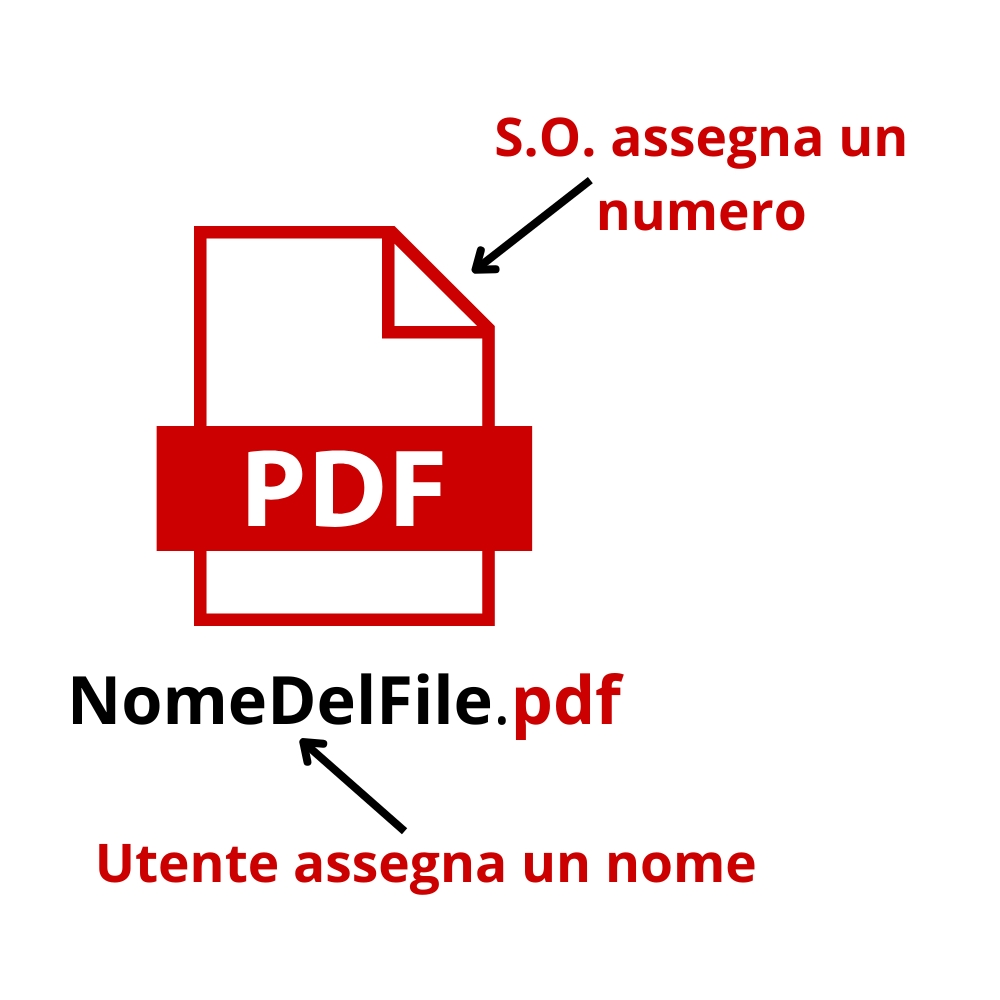
\includegraphics[width=\linewidth]{img/file.jpg}
                \caption{{creata con \href{https://www.canva.com/}{Canva}}}
            \end{figure}
    \end{columns}
\end{frame}

\begin{frame}{CARTELLE}
    \begin{columns}
        \column{.5\textwidth}
            \begin{alertblock}{DEFINIZIONE}
                \begin{minipage}{0.97\linewidth}
                    \justifying
                    Una \textbf{Directory} è un file speciale che contiene informazioni sui file e sulle directory 
                    contenute al suo interno. Come i file normali, anche le directory sono identificate da un nome 
                    e da un numero di identificazione univoco.\\
                    \'E possibile creare una struttura ad albero di directory, inserendo directory all'interno di altre 
                    directory, costruendo così una \textbf{gerarchia di file}.\\
                \end{minipage}
            \end{alertblock}
        \column{.5\textwidth}
            \begin{figure}
                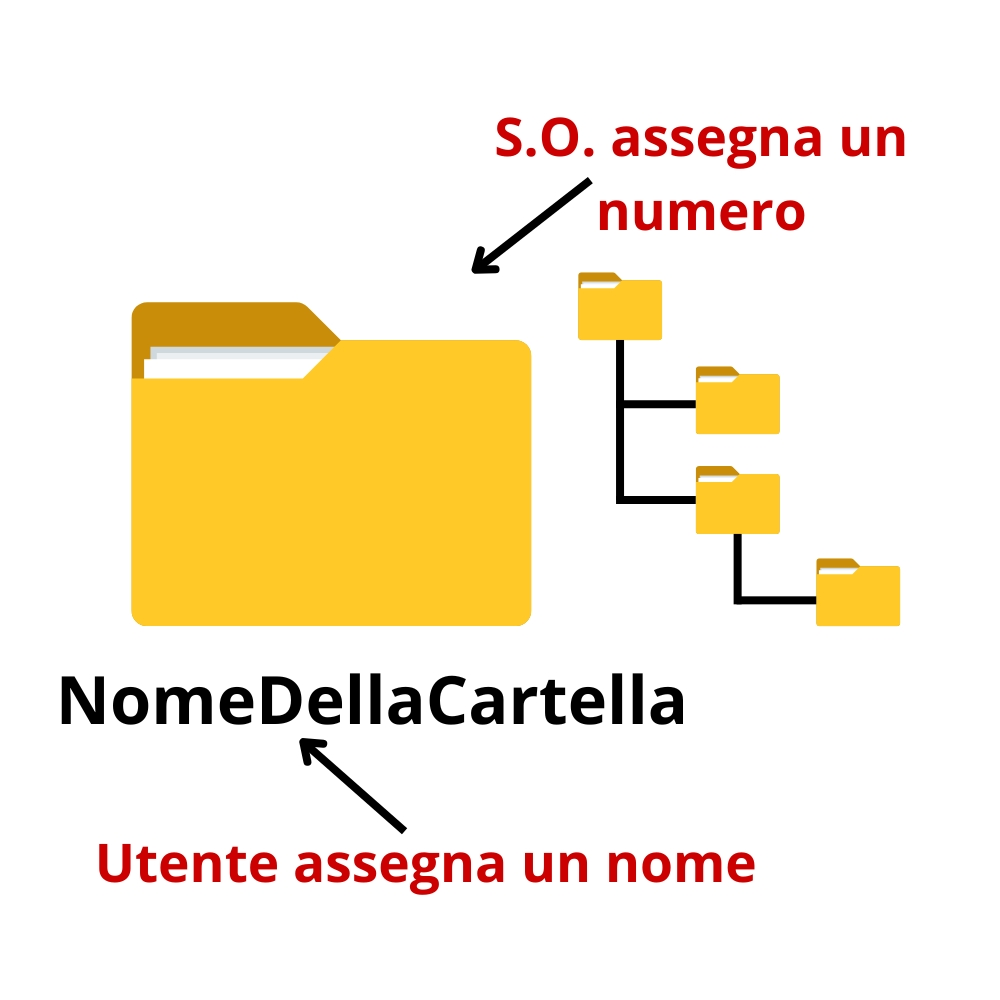
\includegraphics[width=\linewidth]{img/cartella.jpg}
                \caption{{creata con \href{https://www.canva.com/}{Canva}}}
            \end{figure}
    \end{columns}
\end{frame}

\begin{frame}{FILE SYSTEM}
    \begin{alertblock}{DEFINIZIONE}
        \begin{minipage}{0.98\linewidth}
            \justifying
            Il \textbf{File System} è un insieme di strutture dati e algoritmi che permettono di memorizzare, 
            organizzare e gestire i file su un dispositivo di memorizzazione. Il File System si occupa di fornire 
            alle applicazioni un meccanismo per accedere ai file e gestire le operazioni di lettura e scrittura.\\
            \bigskip
            \tiny{\textbf{Curiosità}}\\
            \tiny{\href{https://it.wikipedia.org/wiki/File_system}{Tipologie di File System}}
        \end{minipage}
    \end{alertblock}
\end{frame}

\section{COMPITI E OPERAZIONI DEL FILE SYSTEM}

\begin{frame}{COMPITI E OPERAZIONI DEL FILE SYSTEM}
    \begin{itemize}
        \item \textbf{GESTIRE} in modo ottimale lo \textbf{spazio} disponibile nelle memorie di massa;
        \pause
        \item \textbf{GARANTIRE} all'utente l'\textbf{accesso} ai dati contenuti in uno o più file in modo efficiente;
        \pause
        \item \textbf{FORNIRE} agli utenti meccanismi di \textbf{protezione} dei file (protezione da accessi o scrittura non autorizzati, 
        cancellazione accidentale, ecc...);
        \pause
        \item \textbf{IMPLEMENTARE} le \textbf{operazioni} di uso comune sui file (creazione, copia, \textcolor{red}{\textbf{eliminazione}}, spostamento, ecc...) in modo 
        trasparente per l'utente.
    \end{itemize}
\end{frame}

\begin{frame}{ELIMINAZIONE DI UN FILE}
    \begin{columns}
        \column{.5\textwidth}
            \begin{alertblock}{DEFINIZIONE}
                \begin{minipage}{0.97\linewidth}
                    \justifying
                    L'operazione di \textbf{eliminazione} di un file consiste nel liberare lo spazio di memoria occupato da un file 
                    e renderlo disponibile per la scrittura di un altro file.\\
                    Per liberare lo spazio di memoria associato al file, il sistema operativo deve semplicemente 
                    effettuare un'operazione di \textbf{unlink} sul file, che consiste nel rimuovere il file dal File System, 
                    eliminando l'associazione tra il nome del file e il numero di identificazione univoco.\\
                    \bigskip
                    \tiny{\textbf{Curiosità}}\\
                    \tiny{\href{https://www.garanteprivacy.it/web/guest/home/docweb/-/docweb-display/docweb/1574080}{Come eliminare davvero i dati?}}                                         
                \end{minipage}
            \end{alertblock}
        \column{.5\textwidth}
            \begin{figure}
                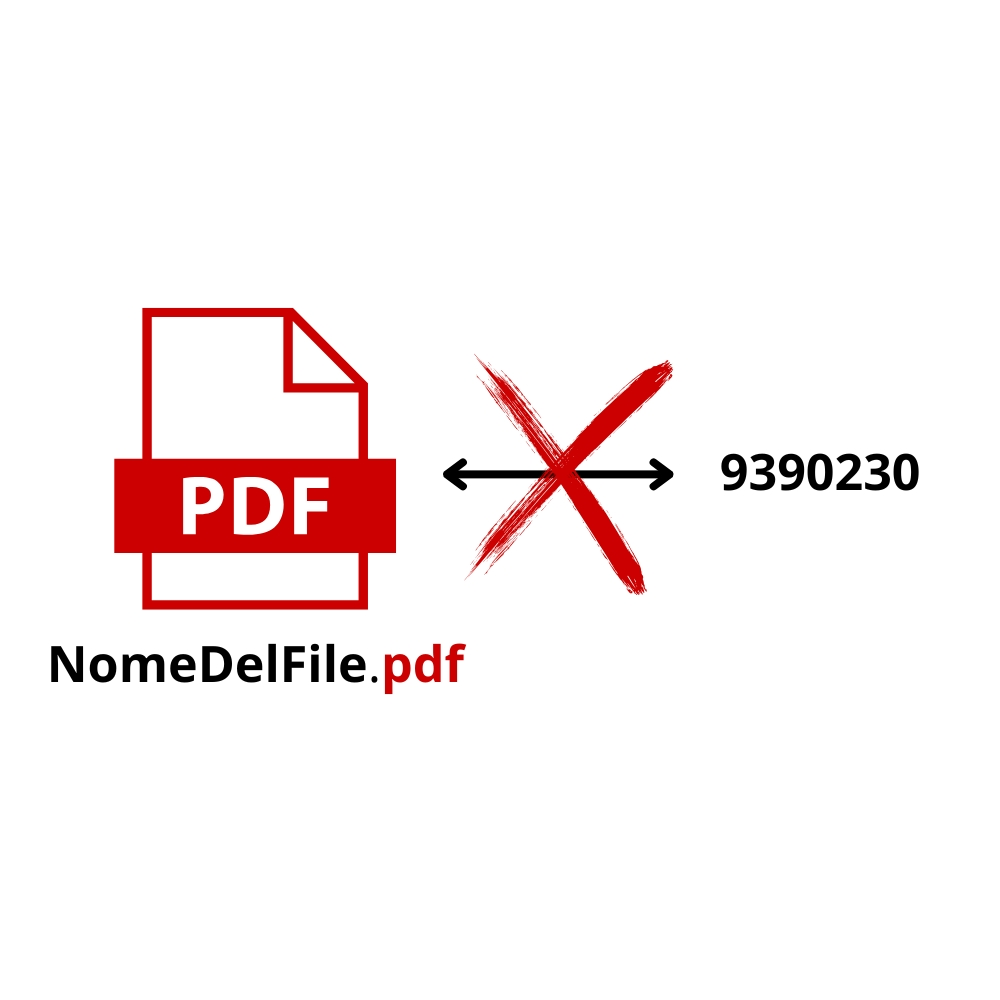
\includegraphics[width=\linewidth]{img/eliminazione.jpg}
                \caption{{creata con \href{https://www.canva.com/}{Canva}}}
            \end{figure}
    \end{columns}
\end{frame}

\end{document}